%!TeX root = ./../MusterAbschlussarbeit.tex

%##########################################################
% Inhalt
%##########################################################

\clearpage
\chapter{Implementation}

\section{Umsetzung in Unity}
Wie wurde Programmiert
UML?
Flussdiagramm?


\subsection{Controller}
Der Controller stellt alle Funktionalitäten bereit, welche gebraucht werden um die Lernumgebung zu initialisieren.
Er besitzt Prefabs des Agents, des GameFields und der Würfel und initialisiert diese zum Start.
Weiterhin implementiert der Controller die Funktionalität der Punktevergabe, welche für eine Mehrspielervariante genutzt werden kann.
Der Controller ist das Parent aller anderen Elemente und so ist er das Zentrale Element der Steuerung. Auch das wiederholte rollen der Würfel wird im Controller angestoßen.
Der Controller war sehr hilfreich beim erstellen paralleler Trainings, da dieser einfach mehrfach in die Szene aufgenommen werden musste um mehrere Spielfelder, welche gleichzeitig bespielt werden zu initialisieren.

<Code ausschnitt?>

\subsection{NumberDice}
Der NumberDice implementiert die Logic, welche für das Würfeln und Visualisieren der Zahlenwürfel benötigt wird.
Die Visualisierung funktioniert mit selbst angefertigten Sprites welche in einem Sortierten Array liegen und je nach gewürfelter Zahl initialisiert und gerendert werden.
Beim wiederholten Würfeln, wird das initialisierte Sprite destroyed und ein neues erzeugt.
Damit ist gewährleistet, dass immer das aktuelle Würfelergebnis angezeigt wird.
Die Zahl des Würfels wird als Integer wert gespeichert, wobei er die Zahlen 1-6 annehmen kann.
Die Zahl sechs entspricht dem Zahlenjoker.

<Code>
<Bild der Sprites>

\subsection{ColorDice}
Wie der Zahlenwürfel implementiert der ColorDice die Funktionalität des Würfelns der Farben.
Diese werden als String dargestellt und kann folgende Werte annehmen: \{'blue', 'green','red', 'yellow', 'orange', 'joker'\}
Zur Visualisierung wird ein Sprite erstellt, was in der gewürfelten Farbe eingefärbt wird.
Ein schwarzes Feld entspricht dem gewürfelten Farbjoker.

<Code>


\subsection{GameField}
Das GameField stellt das tatsächliche Spielfeld dar.
Es implementiert die benötigten Methoden um die SquareFields zu verwalten und rückzusetzen.
Außerdem wird die Anzahl der Joker in ihm gehalten.

Funktionalitäten:
\setlist{noitemsep}
\begin{itemize}
	\item  Visualisierung des Spielfeldes
    \item  Aktualisieren der Gruppen aller Felder
    \item  Abkreuzen der Felder
    \item  Berechnen der validen Nachbarn der Felder
    \item  Berechnen der verbleibenden Felder einer bestimmten Farbe
    \item  Rückgabe der validen Felder für die aktuell gewählten Würfel.
    \item  Reduzieren der verbleibenden Joker
    \item  Rücksetzen der Felder um ein neuest Spiel zu Starten
\end{itemize}

\subsection{FieldSquare}

Die FieldSquares stellen die einzelnen Teilfelder des Spielfeldes dar.
Gehaltene Informationen:
\setlist{noitemsep}
\begin{itemize}
    \item Feld ist ein Sternfeld    -> bool
    \item Farbe des Feldes          -> string
    \item Feld ist ausgefüllt       -> bool
    \item Feld ist verfügbar        -> bool
    \item Clustergröße              -> int
    \item X Koordinate des Feldes   -> int
    \item Y Koordinate des Feldes   -> int
\end{itemize}

\subsection{Visualisierung}
Die Visualisierung des Spielfeldes erfolgt über ein angefertigtes Prefab. In diesem wurden die 105 Kästchen in einem Raster von 15x7 instanziiert und manuell mit den Informationen versehen. Dieses manuell angefertigte Spielfeld wurde als Prefab gespeichert und dient als Umgebung für den Agenten.
Zu Beginn des Spiels, werden die Felder in die Farben der hinterlegten Information in den richtigen Farben eingefärbt. Ausgefüllte Kästchen werden grau eingefärbt, diese Funktionalität wird im Fieldsquare Prefab ausgeführt.

<Code instanziierung der Felder?>

<Code einfärben der Felder>

\subsection{Agent}

\section{Implementierung des Agenten}
Der Agent ist die Schnittstelle zwischen dem Environment und dem RL.
Dem Agent werden alle nötigen Informationen des Spielfeldes übergeben. Diese werden in ein Neuronales Netz übertragen, welches wiederum die Ausgabewerte in einem Vektor zurück an den Agent leitet.
Anschließend wird der Vektor verarbeitet und die gewählten Aktionen werden ausgeführt.
Für gute Aktionen erhält der Agent positive Rewards, bei schlechten Aktionen wird der Zug übersprungen.

\subsection{Observations}
Zu Beginn jeder Episode (=SChritt) muss dem Agenten der aktuelle Zustand des Feldes übermittelt werden, aus welchem er die bestmögliche Option für einen Zug berechnet. In der ML Agents Bibliothek gibt es hierfür eine vorgefertigte Methode mit dem Namen CollectObservations.
Die bearbeitet einen Observationsvektor zu welchem die Informationen hinzugefügt werden.
Wärend des Trainings eines Neuronalen Netzes, muss die Anzahl der Observations gleich bleiben. Das bedeutet es ist nicht ohne weiteres möglich ein Model auf unterschiedlichen Spielfeldern zu trainieren, da sic hso die Anzahl der Observations unterscheiden würden.


Aufbau der Observations:
\setlist{noitemsep}
\begin{itemize}
\item Anzahl der verbleibenden Joker: int[0-11]
\item Anzahl der gespielten Runden: int[0-30]
\item Ergebnis der Zahlenwürfel: int[0-5]
\item Ergebnis der Farbwürfel: Vector6[0,1]
\end{itemize}

Für jedes Feld:
\setlist{noitemsep}
\begin{itemize}\subsection{Bewertungsmetriken für RL-Agenten}
\item Farbe des Feldes: Onehot vector5[0,1]
\item Ist das Feld verfügbar: bool
\item Ist das Feld bereits abgestrichen: bool
\item Ist das Feld ein Sternfeld:  bool
% \item Clustergröße des Feldes: int {1-5}
% \item Koordinate des Feldes: Vector2(int, int) 0-7 / 0-15
\end{itemize}

<skript Collect Observations>

//TODO 2 verschiedene Varianten was mach ich damit?

\subsection{Actions}
Anhand der Observations berechnet das Neuronale Netz einen Ausgabevektor. Mit diesem führt der Agent nun bestimmte Aktionen aus und versucht sein Ergebnis (Rewards) zu maximieren.
Anhand der gesammelten Rewards wird das Neuronale Netz nun angepasst um das bestmögliche Ergebnis zu erreichen.


Aufbau Actionbuffer:
\setlist{noitemsep}
\begin{itemize}
\item Index des gewählten ZahlenWürfels: int (0-1)
\item Index des gewählten Farbwürfels: int(0-1)
\item Jokerzahl int 0-4
\item X Koordinate des gewählten Feldes: int (0-14)
\item Y Koordinate des gewählten Feldes: int(0-7)
\item 4 x Continous Action für die Auswahl der Nachbarn
\end{itemize}

what to do unterscheidliche actions


\newpage
\subsection{Erklärung des Alghorhytmus mit dem Beispielhaften Ausgabevektor (1,1,0,3,4, 0.6, 0.5, 0.4, 0.8)}
Die ersten beiden Stellen des Ausgabevektors entsprechen den gewählten Würfeln.

Im ersten Schritt werden alle Feldes des Spielfedes untersucht, ob sie ein valides Ziel für das gewürfelte Ergebnis bilden.
Die ergibt sich aus der Gruppe der Spielfelder, der Farbe und ob das Kästchen verfügbar ist.
Valide Felder werden in eine Liste (availableFields) aus Verfügbaren Feldern geschrieben.

\begin{figure}[!h]
	\centering
	\includegraphics[width=0.5\textwidth]{Bilder/Erklärung_Alghorhitmus_1.png}
	\caption{Valide Felder für das gewählte Würfelergebnis wurden markiert}
\end{figure}

Anschließend wird geprüft, ob die gewählten Koordinaten in availableFields vorhanden sind.
Wenn nein wird die Episode abgebrochen und der Agent überspringt seinen Zug.
Sofern der Agent ein valides Feld gewählt hat, wird dieses in eine weitere Liste (pickedFields) geschrieben und benachbarte Felder der selben Gruppe werden zurückgegeben.

\newpage
\begin{figure}[!h]
	\centering
	\includegraphics[width=0.5\textwidth]{Bilder/Erklärung_Alghorhitmus_2.png}
	\caption{Feld(3,4) wird in die pickedField Liste aufgenommen und benachbarte Felder werden zurückgegeben.}
\end{figure}

Im nächsten Schritt wird jedem der verfügbaren Nachbarn abhängig der Gesamtanzahl ein Wertebereich zwischen 0 und 1 zugewiesen. Anhand des discreten Wertes des Ausgabevektors wird das Zugehörige Feld in pickedFields geschrieben.
\setlist{noitemsep}
\begin{itemize}
\item Feld(3,5) 0 bis 0.33
\item Feld(4,4) 0.33 bis 0.66
\item Feld(3,3) 0.66 bis 0.99
\end{itemize}

\begin{figure}[!h]
	\centering
	\includegraphics[width=0.5\textwidth]{Bilder/Erklärung_Alghorhitmus_3.png}
	\caption{Feld(4,4) ist das nächste gewählte Feld und wird in pickedFields aufgenommen}
\end{figure}

Für alle Feldes in Picked Field werden die benachbarten Felder zurückgegeben und der vorherige Schritt wiederholt.
Wenn so viele Felder gewählt wurden, wie erwürfelt wurden, werden die Felder anschließend ausgefüllt und auf Rewards überprüft.

\begin{figure}[!h]
	\centering
	\includegraphics[width=0.5\textwidth]{Bilder/Erklärung_Alghorhitmus_4.png}
	\caption{Felder wurden gewählt und ausgefüllt}
\end{figure}


\newpage


\section{Trainingsversuche}
\subsection{Trainingsversuche}

Aufbau Actionbuffer bis dato -> würfel, würfel, feldIndex, feldIndex , feldIndex ,feldIndex, feldIndex (feldIndex int)
In den ersten Trainings soltle der Agent Würfel und anschließend zufällige Felder wählen.
Danach wurde überprüft ob alle ausgewählten Felder folgende Kriterien erfüllten:
\setlist{noitemsep}
\begin{itemize}
\item alle Felder verfügbar
\item alle Felder benachbart
\item alle Felder der selben farbe
\end{itemize}

Illegale Züge wurden bestraft (negative Rewards) und wurden nicht ausgeführt.
Da der Agent Anfangs zufällige Felder auswählt, hatte es zur Folge, dass nahezu keine Spielzüge getätigt wurden.
Dies führte dazu, dass das Spiel nicht gespielt wurde.
Dementsprechend war das Training auf diese Weise nicht erfolgreich und musste überarbeitet werden.




\subsection{Training des Agenten mit Zusatz Belohnungen}
In den Bereits erläuterten Trainingsversuchen, bekam der Agent für vermeintlich gute Züge eine Belohnung und für schlechte Züge eine Bestrafung.

- Für das Abkreuzen von Feldern 0.02f pro feld
- falls ein gesammmtes Cluster abgekreuzt wird -> 0.04 pro feld
- wahl eines Würfelpaars für das es keine legalen Züge gibt -> -50.0f
- Wahl eines Jokers obwohl keine Joker verfügbar sind -> -50.0f

Die Belohnungen führten dazu, dass der Agent nicht Versuchte Spalten abzukreuzen, da er das abkreuzen von Clustern für deutlich effizienter hielt um siene Belohnungen zu maximieren.
Obwohl die Belohnungen für Erreichte Spalten oder komplett ausgefüllte Farben mehr Punkte ergaben.


\begin{figure}[!t]
    \centering
    \includegraphics[scale=0.6]{Bilder/average_points.png}
    \caption{Das Logo von Informatik und Medien }
\end{figure}

\begin{figure}[!t]
    \centering
    \includegraphics[scale=0.6]{Bilder/average_rewards.png}
    \caption{Das Logo von Informatik und Medien }
\end{figure}

Die Grafiken zeigen deutlich, dass je länger der Agent tranierte desto kleiner die Durchschnittlichen Punkte pro Spiel wurden.
Dies spricht dafür, dass es zum sogenannten 'reward hacking' gekommen ist. Dieses Phänomen tritt auf, wenn der Agent sein eigentliches Ziel nicht erreichen kann, da er eine andere (falsche) Strategie erlernt, welche nicht zum eigentlichen Ziel führt. Ursache hierfür ist, dass der Agent sein eigentliches Ziel (das ausfüllen von Spalten) nie erreicht und somit nicht erlernt.



\subsection{Training des Agenten ohne Zusatz Belohnungen}
Da auch der vorhergehende Versuch keinen klaren trend zu Verbesserung aufzeigte, entschied ich mich, einzig die Punktebewertung des Spiel als Rewards zu benutzen.
Auf diese Weise bekommt der Agent nur Rewards für Punkte welche er auch für das spielen erhält. Auf diese Weise, kann er sich keine 'Falschen' Strategien erarbeiten, welche aus falsch festgelegten Rewards resultieren.

Rewards gibt es nun für:
Ausfüllen von 'Sternfeldern' -> 2.0f
Auffüllen einer kompletten Spalte -> (je nach Spalte 5-1)
Ausfüllen einer kompletten Farbe -> (5 Punkte)
Übrig gebliebene Joker nach Ablauf der 30 Spielrudnen -> 1 Punkt pro Joker

\subsection{Verbesserung des Trainings}
Verlängerung der Spieldauer

Training mit Speziellen Feldern

Verkleinerung des Feldes

Änderung der Policy

\subsection{Training Auswahl Initiales Feld}
Da der Agent keine großen Fortschritte erzielen konnte, entscheid ich den Agenten das erste Feld durch Koordinaten zu wählen.
Dies setzte Vorraus, dass die Koordinaten der einzelnen Felder in die Observations mit aufgenommen werdne musste und die Observations noch größer wurden.
Damit der Agent lernen kann, welche Kooordinaten zu welchen Feldern gehören, entschied ic hmic hdazu ihn auf einem Spielfeld trainieren zu lassen, wo alle Teilfelder verfügbar sind.
Rewards wurden vergeben für Valide ausgewählte Felder, in Abhängigkeit der gewürfelten Zahlen.

Im nächsten Schritt wird dieses vortrainierte NN genutzt um das Spiel mit richtigen Regeln zu spielen.



Zusammenhängende Ergebnisse werden vorteilhaft in Form von Tabellen (wie in \ref{TabLaufzeiten}) dargestellt.

\begin{table}[h!]
	\begin{center}
        \caption{Laufzeiten in sec, gemessen mit einem Intel xy-8 Ghz Prozessor}\label{TabLaufzeiten}
		\begin{tabular}{|c||c|c|c|}
			\hline 
			& Verfahren X & Verfahren Y & Verfahren Z \\ 
			\hline 
			\hline 
			\hspace{.1cm}
			Problem A & 300 & 340 & 210 \\ 
			\hline 
			\hspace{.1cm}
			Problem B & 730 & 580 & 540 \\ 
			\hline 
			\hspace{.1cm}
			Problem C & 610 & 420 & 440 \\ 
			\hline 
			\hspace{.1cm}
			Problem D & 895 & 790 & 520 \\ 
			\hline 
		\end{tabular} 
	\end{center}
\end{table}


Funktionale Zusammenhänge hingegen lassen sich in Form von Diagrammen oder Grafiken (Siehe \ref{fig:Abbildung1}) darstellen.


\begin{figure}[!htb]
	\centering
	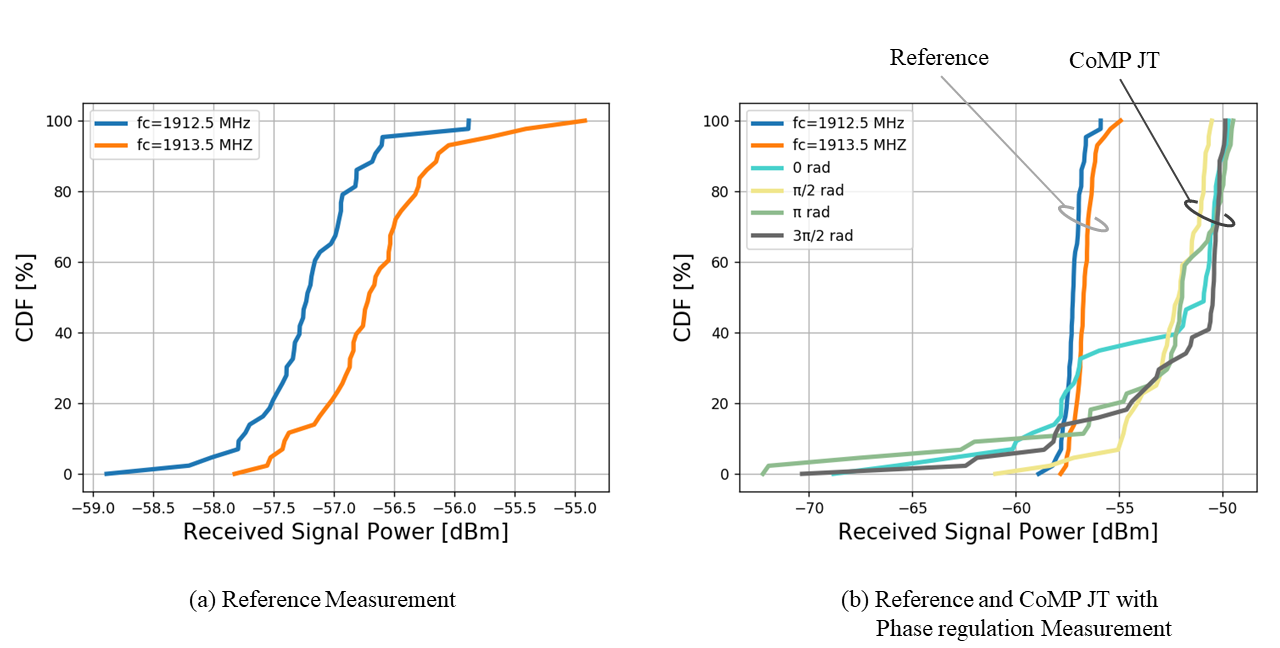
\includegraphics[width=1\textwidth]{Bilder/Abbildung1}
	\caption{Statistical analysis of the received power}
	\label{fig:Abbildung1}
\end{figure}

Ein guter Ergebnisteil erfordert Literaturzitate (vielleicht auch gar keine) und die Bekanntgabe des Ergebnisses sollte von einer Interpretation und Diskussion begleitet werden. 


\newpage

\underline{Aber \textbf{mindestens} folgende Punkte}\\
Inhalt des vierten Kapitels (im Allgemeinen):
\begin{itemize}
    \item Setzen Sie nun den Plan aus dem dritten Kapitel wenigstens prototypisch um
    \item Ziel ist es Ihre Überlegungen und Darlegungen zu beweisen
    \item Diskutieren von Problemen
    \item Zusätzlich zu der Umsetzung bedarf es (von Ihnen zu definierender) Tests, um die Funktionalität zu beweisen
    \begin{itemize}
        \item Laufzeittests, Lasttests, etc.
        \item Produzieren Sie Ergebnisse um zu zeigen, dass Ihr Ansatz funktioniert und besser/schlechter ist
        \item \glqq schlechter\grqq{} sein, bedeutet nicht, dass Ihre Arbeit schlecht ist! Am Ende zählt Ihr Ansatz und die Idee
    \end{itemize}
\end{itemize}
